\documentclass[a4paper, 11pt, final, garamond]{book}
\usepackage{cours-preambule}

\raggedbottom

\makeatletter
\renewcommand{\@chapapp}{Travaux pratiques -- TP}
\makeatother

\let\SavedIndent\indent
\protected\def\indent{%
  \begingroup
    \parindent=\the\parindent
    \SavedIndent
  \endgroup
}
\setlength{\parindent}{0pt}

\begin{document}
\setcounter{chapter}{4}

\chapter{Oscilloscope et trac\'e de caract\'eristiques}
\section{Objectifs}

\begin{itemize}
    \item Se familiariser avec le GBF et l'oscilloscope numérique.
    \item Réaliser des montages simples d'électricité.
    \item Mesurer la résistance d'entrée $R_{e}$ d'un oscilloscope et la
        résistance de sortie $R_{s}$ d'un GBF.
    \item Tracer une caractéristique de dipôle en utilisant un transformateur
        d'isolement.
\end{itemize}

\section{S'approprier}

\subsection{Résistances d'entrée et de sortie}

Nous avons vu en TD la méthode dite de la «~demi-tension~» qui permet de mesurer
la résistance d'entrée et de sortie d'un appareil (cf.\ exercice I TD 2, fait
\textit{via} la puissance)

\subsubsection{Résistance de sortie du générateur basse fréquence (GBF)}

\begin{wrapfigure}[6]{R}{0.35\textwidth}
\vspace{-35pt}
  \begin{center}
    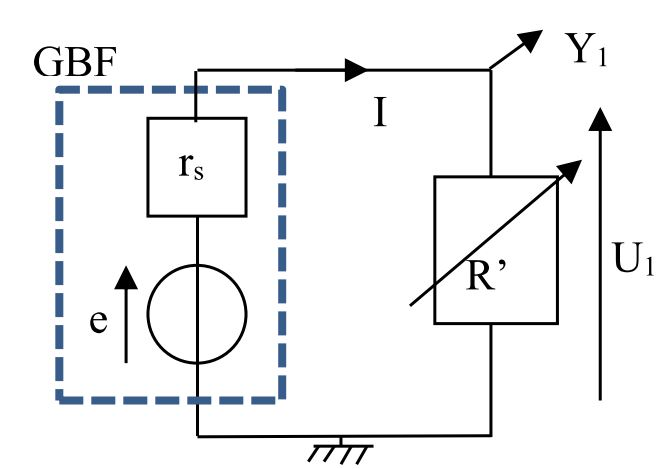
\includegraphics[width=0.35\textwidth]{res_entree}
  \end{center}
\end{wrapfigure}

Le GBF est un générateur réel pouvant être modélisé comme une association série
d'un générateur idéal de tension de force électromotrice $e$ associé à une
résistance de sortie $r_{s}$ (modèle de Thévenin). Comme vu en cours, on branche
le GBF sur une résistance variable $R'$ puis on mesure la tension $U_1$ aux
bornes de $R'$. Montrer que lorsque $U_1 = e/2$, alors $R' = r_{s}$. En déduire
une méthode simple de mesure expérimentale de $r_{s}$.

\medskip
\vspace{10pt}

\begin{instruc}{Aide}
    Afin de mesurer $U_1$, l'oscilloscope se branche entre la masse (reliée à la
    borne noire de l'oscilloscope) et le nœud $Y_1$ (relié à la borne rouge de
    l'oscilloscope). Notez que dans un circuit, \textbf{la masse est un nœud
    commun à tous les appareils branchés}.
    Par conséquent, la borne noire du GBF ainsi que les deux bornes noires de
    l'oscilloscope doivent être impérativement reliées entre elles. Si ce n'est
    pas le cas, votre montage ne fonctionnera pas.
\end{instruc}

\subsubsection{Résistance d'entrée de l'oscilloscope}

\begin{wrapfigure}[10]{r}{0.4\textwidth}
    \vspace{-20pt}
    \begin{center}
        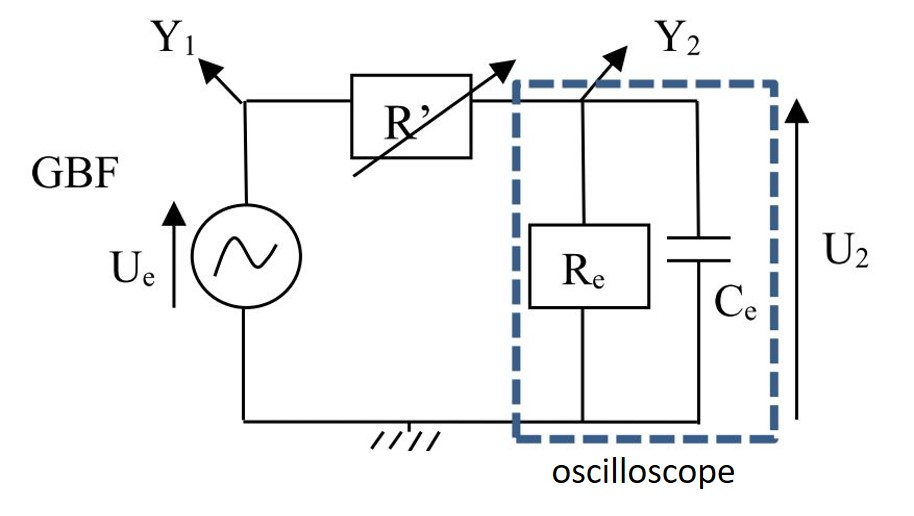
\includegraphics[width=0.4\textwidth]{res_sortie}
    \end{center}
    \vspace{-30pt}
\end{wrapfigure}

L'entrée d'un oscilloscope est assimilable à une résistance d'entrée $R_{e}$ en
dérivation avec une capacité $C_{e}$. À basse fréquence, le condensateur est
assimilable à un interrupteur ouvert si bien que l'on peut dans un tel régime
négligé sa présence. Montrer alors, en vous aidant du schéma, que la tension
$U_2$, mesurée par l'oscilloscope (modélisée par une résistance et une capacité
en parallèle), est égale à $U_{e}/2$ lorsque $R' = R_{e}$. En déduire une
méthode simple de mesure expérimentale de $R_{e}$. Remarquez que, contrairement
à ce qui est fait dans le cours, la résistance de sortie du GBF n'apparaît pas.
Elle est en réalité très faible devant les autres résistances $R_{e}$ et $R'$ et
sera donc négligée.

\subsection{Mesures avec un oscilloscope}

À partir du menu mesure, l'oscilloscope est capable de réaliser des mesures
automatiques des principales caractéristiques des signaux électriques. Vous
pourrez en particulier afficher~:

\begin{itemize}
    \item la période et la fréquence du signal~;
    \item la tension crête-crête $u_{\rm pp}$ du signal (valeur mesurée entre le
        maximum et le minimum du signal)~;
    \item la tension efficace $u_{\rm eff}$ définie par
        \encadre{$S_{\rm eff} = \sqrt{ \left\langle s^2(t) \right\rangle}
                              = \sqrt{\frac{1}{T}\int_{t_0}^{t_0+T} s^2(t) \dt}$}
\end{itemize}

\begin{minipage}{0.45\linewidth}
    L'amplitude $A$ d'un signal (qui intervient dans l'expression d'un signal
    sinusoïdal selon $s(t) = A \cos(\omega t + \varphi)$) est liée à $V_{\rm
    pp}$ selon

    \encadre{$A = u_{\rm pp}/2$}
\end{minipage}
\hfill
\begin{minipage}{0.45\linewidth}
    Par ailleurs, pour un signal sinusoïdal, \textbf{et uniquement pour un
    signal sinusoïdal} la tension efficace s'écrit~:

    \encadre{$u_{\rm eff} = u_{\rm pp}/\sqrt{2} = \sqrt{2} A$}
\end{minipage}

\begin{NCror}[width=\linewidth]{Attention}
    Pour toute mesure, vérifier que la source du menu mesure correspond bien à
    la courbe sur laquelle vous faites des mesures.
\end{NCror}

\subsection{Utilisation des oscilloscopes}
\subsubsection{Imprimer une courbe avec un oscilloscope \texttt{Rigol}}

\begin{enumerate}
    \item Allumer l'ordinateur et se connecter au réseau.
    \item Puis, programme, discipline, physique-chimie, physique, oscillo
        \texttt{rigol}.
    \item \texttt{Tools}, \texttt{connect to oscillo}, puis \texttt{refresh}.
    \item Passer en noir et blanc (\texttt{B \& W}) et enfin \texttt{print}.
\end{enumerate}


\subsubsection{Imprimer une courbe avec un oscilloscope \texttt{Tektronix}}

\begin{enumerate}
    \item Ouvrir \texttt{Open Choice Desktop}. Sélectionner \texttt{instrument
        USB} puis \texttt{Afficher écran}.
    \item Copier vers le presse-papier. Ouvrir \texttt{paint} et coller.
    \item Puis cliquer droit, inverser les couleurs.
    \item Sélection rectangulaire, pour ne garder que les oscillogrammes et les
        réglages de l'oscilloscope.
    \item Copier~; Basculer dans \texttt{libre-office} ou \texttt{word} et
        Coller~;
    \item Faire une belle mise en page et mettre des titres et commentaires
        éventuels. Puis imprimer.
\end{enumerate}

\section{Réaliser~: Résistances d'entrée et de sortie}
\subsection{Mesure de la résistance de sortie du GBF}

\begin{enumerate}
    \item Réaliser le montage vu dans la partie \textit{S'approprier} pour une
        fréquence d'environ $\SI{100}{Hz}$ et commencer avec $R'$ infinie, donc
        débranchée.
    \item Mesurer alors $U_1$ grâce à l'oscilloscope, et régler le
        \texttt{level} du GBF (bouton DC offset enfoncé) pour obtenir une
        tension crête-crête de $\SI{2}{V}$. Cette tension correspond à la
        tension à vide $e$ du générateur. En effet, à vide, c'est-à-dire pour
        $R'$ infinie, le courant est nul et donc la tension relevée est
        directement égale à $e$.
    \item Brancher la boîte de résistances variables $R'$ et l'ajuster pour
        avoir $U_1 = e/2$.
    \item En déduire l'ordre de grandeur de la résistance de sortie $r_{s}$ du
        GBF.
    \item Cette valeur est-elle cohérente avec les indications inscrites sur la
        sortie du GBF~?
\end{enumerate}

\vspace{-0.6cm}

\subsection{Mesure de la résistance d'entrée de l'oscilloscope (modèle)}

\begin{enumerate}
    \item Prendre la notice de l'oscilloscope dont vous disposez, vérifier les
        valeurs de $R_{e}$ et $C_{e}$ appelées \textit{input impedance} en
        anglais.
    \item Mesurer d'abord la tension $U_{e}$ en connectant directement
        l'oscilloscope au générateur (cela revient à prendre une résistance $R'$
        nulle, assimilable à un fil donc).
    \item Réaliser ensuite le montage présenté dans la partie
        \textit{S'approprier}.
    \item $U_{e}$ étant fixé ($\SI{2}{V}$ crête-crête), faire varier $R'$
        jusqu'à ce que la tension aux bornes de l'oscilloscope ($U_2$) soit
        égale à la moitié de la tension du générateur $U_{e}$. Vous pouvez
        utiliser le menu mesure pour obtenir la valeur des deux tensions.
    \item En déduire l'ordre de grandeur de la résistance d'entrée $R_{e}$
        expérimentale de l'oscilloscope.
\end{enumerate}

\section{Valider~: Effets des résistances d'entrée et de sortie}
\subsection{Effet de la résistance de sortie du GBF}

\begin{enumerate}
    \item Brancher l'oscilloscope aux bornes du GBF (toujours réglé à une
        fréquence de $\SI{100}{Hz}$) et régler le \texttt{level} de celui-ci
        pour obtenir une tension crête-crête de $\SI{2}{V}$. Comme précédemment,
        nous mesurons ici la tension à vide $e$ du GBF.
    \item Brancher aux bornes du GBF deux résistances identiques de $R_1 = R_2 =
        \SI{47}{\Omega}$ en série puis relever à l'aide de l'oscilloscope la
        tension $U_1$ aux bornes de l'une d'elle.
    \item En appliquant le principe du pont diviseur de tension, que devrait
        valoir $U_1$~? Est-ce la valeur que vous relevez~?
    \item Expliquez cet écart en considérant la résistance de sortie du GBF.
    \item Comment choisir $R_1$ et $R_2$ pour que l'on puisse négliger l'effet
        de la résistance de sortie du GBF~? Reproduire le montage précédent en
        utilisant désormais $R_1 = R_2 = \SI{10}{k\Omega}$. Montrer qu'alors
        $U_1$ prend la valeur attendue.
\end{enumerate}

\subsection{Effet de la résistance d'entrée de l'oscilloscope}

\begin{enumerate}
    \item Brancher l'oscilloscope aux bornes du GBF (toujours réglé à une
        fréquence de $\SI{100}{Hz}$) et régler le \texttt{level} de celui-ci
        pour obtenir une tension crête-crête de $\SI{4}{V}$. Comme précédemment,
        nous mesurons ici la tension à vide $e$ du GBF.
    \item Brancher aux bornes du GBF deux résistances identiques de $R_1 = R_2 =
        \SI{1}{M\Omega}$ en série puis relever à l'aide de l'oscilloscope la
        tension $U_1$ aux bornes de l'une d'elle.
    \item La tension $U_1$ obtenue est-elle conforme à vos attentes~? Expliquez
        cet écart en tenant compte de la résistance d'entrée de l'oscilloscope.
    \item Comment choisir $R_1$ et $R_2$ pour que l'on puisse négliger l'effet
        de la résistance d'entrée de l'oscilloscope~? Reproduire le montage
        précédent en utilisant désormais $R_1 = R_2 = \SI{10}{k\Omega}$. Montrer
        qu'alors $U_1$ prend la valeur attendue.
\end{enumerate}

\section{Conclure}

Résumer les recommandations pratiques que vous avez pu déduire de ce TP afin de
réaliser des mesures correctes en électricité.

\end{document}
